% Biên dịch: python report/build.py (sinh lại số liệu từ results/, rồi chạy XeLaTeX hai lần).
% Mọi con số trong bài đến từ report/generated/*.tex do report/make_assets.py sinh ra
% từ results/. Không gõ tay số liệu vào đây.
\documentclass[11pt,a4paper]{article}

\usepackage{fontspec}
\setmainfont{Times New Roman}
\usepackage[vietnamese]{babel}
\usepackage[margin=2.2cm]{geometry}
\usepackage{graphicx}
\usepackage{booktabs}
\usepackage{amsmath}
\usepackage{amssymb}
\usepackage{caption}
\usepackage[hidelinks]{hyperref}
\usepackage{xcolor}

\graphicspath{{generated/}}
\captionsetup{font=small,labelfont=bf}
\setlength{\parskip}{0.4em}
\setlength{\parindent}{0pt}

% Chỗ cần tự viết thêm. \showtodofalse để ẩn hết khi nộp.
\newif\ifshowtodo\showtodofalse
\newcommand{\todo}[1]{\ifshowtodo{\color{red}\small[TODO: #1]}\fi}

\newcommand{\bestacc}{98{,}85\%}
\newcommand{\bestmodel}{SVM (RBF)}
\newcommand{\bestfeatures}{Hình dạng + Màu + Kết cấu}
\newcommand{\bestdims}{57}
\newcommand{\beststd}{0{,}43}
\newcommand{\shapeonlyacc}{86{,}26\%}
\newcommand{\shapeonlyrf}{90{,}25\%}
\newcommand{\shapecoloracc}{97{,}59\%}
\newcommand{\allgroupsacc}{98{,}79\%}
\newcommand{\colorgain}{11{,}33\%}
\newcommand{\texturegain}{1{,}26\%}
\newcommand{\veindelta}{-0{,}05\%}
\newcommand{\holdoutacc}{98{,}95\%}
\newcommand{\holdouttotal}{477}
\newcommand{\holdouterrors}{5}
\newcommand{\shapedims}{17}
\newcommand{\colordims}{18}
\newcommand{\texturedims}{22}
\newcommand{\veindims}{7}
\newcommand{\totaldims}{64}
\newcommand{\ccacolortexture}{0{,}975}
\newcommand{\ccatextureshape}{0{,}949}
\newcommand{\ccacolorshape}{0{,}892}
\newcommand{\rtwocolortexture}{0{,}451}
\newcommand{\rtwotexturecolor}{0{,}470}
\newcommand{\mishape}{1{,}273}
\newcommand{\micolor}{0{,}814}
\newcommand{\mitexture}{0{,}990}
\newcommand{\mivein}{0{,}916}
\newcommand{\impshape}{0{,}0876}
\newcommand{\impcolor}{0{,}0459}
\newcommand{\imptexture}{0{,}0245}
\newcommand{\pcavarshape}{61{,}8}
\newcommand{\ldavarshape}{77{,}0}
\newcommand{\ldaknnshapetwo}{55{,}8\%}
\newcommand{\ldaknnshapeten}{88{,}7\%}
\newcommand{\pcavarbest}{44{,}6}
\newcommand{\ldavarbest}{61{,}9}
\newcommand{\ldaknnbesttwo}{55{,}3\%}
\newcommand{\ldaknnbestten}{97{,}8\%}
\newcommand{\ldaoutliers}{\emph{deodar}, \emph{Japanese maple}, \emph{castor aralia}}
\newcommand{\invcontrol}{0{,}9895}
\newcommand{\invtexid}{0{,}8323}
\newcommand{\invtexrotninety}{0{,}8323}
\newcommand{\invtexrotfifteen}{0{,}3354}
\newcommand{\invshapeid}{0{,}8721}
\newcommand{\invshaperotninety}{0{,}8029}
\newcommand{\invshapescale}{0{,}7925}
\newcommand{\invhsvid}{0{,}8616}
\newcommand{\invhsvdark}{0{,}3040}
\newcommand{\invrgbdark}{0{,}1866}
\newcommand{\invhsvnoise}{0{,}4319}
\newcommand{\invrgbnoise}{0{,}7568}
\newcommand{\invshapenoise}{0{,}8470}
\newcommand{\invcombonoise}{0{,}4382}
\newcommand{\invshapeoccl}{0{,}7002}
\newcommand{\invcombooccl}{0{,}0419}
\newcommand{\driftglcmninety}{0{,}00}
\newcommand{\driftlbpninety}{0{,}01}
\newcommand{\driftglcmfifteen}{0{,}33}
\newcommand{\driftlbpfifteen}{0{,}72}
\newcommand{\driftsmoothscale}{8{,}13}
\newcommand{\driftsmoothninety}{0{,}39}
\newcommand{\veinotsusvm}{-0{,}05}
\newcommand{\veinotsusvmp}{0{,}70}
\newcommand{\veinotsuknn}{+0{,}31}
\newcommand{\veinotsuknnp}{0{,}46}
\newcommand{\veinpctsvm}{+0{,}10}
\newcommand{\veinpctsvmp}{0{,}65}
\newcommand{\veinpctknn}{+0{,}89}
\newcommand{\veinpctknnp}{0{,}07}
\newcommand{\veinfrangisvm}{-0{,}05}
\newcommand{\veinfrangisvmp}{0{,}85}
\newcommand{\veinfrangiknn}{+0{,}73}
\newcommand{\veinfrangiknnp}{0{,}06}


% babel-vietnamese đặt tiêu đề danh mục là "Tài liệu"; văn bản học thuật dùng "Tài liệu tham khảo".
\addto\captionsvietnamese{\renewcommand{\refname}{Tài liệu tham khảo}}

\title{\vspace{-1.5cm}Phân lớp lá cây trên bộ dữ liệu Flavia\\
\large Kết hợp đặc trưng hình dạng, màu sắc, kết cấu và gân lá với SVM}
\author{Học viên thực hiện: Võ Hoàng Khang \quad MSHV: 25C01034\\[0.3em]
\small Mã nguồn: \url{https://github.com/vo-hoang-kh4ng/Leaf-Segmentation}}
\date{\today}

\begin{document}
\maketitle
\vspace{-0.8cm}

\begin{abstract}
\noindent
Báo cáo trình bày một quy trình thị giác máy tính cổ điển cho bài toán phân lớp 32 loài lá cây
trên bộ dữ liệu Flavia (1907 ảnh), gồm ba bước: phân đoạn lá khỏi nền, trích xuất bốn nhóm đặc
trưng thủ công độc lập (hình dạng, màu sắc, kết cấu, gân lá) và phân lớp bằng các bộ phân lớp
truyền thống. Bên cạnh việc cài đặt lại phương pháp, báo cáo thực hiện ba thực nghiệm phân tích:
(i) phân tích loại bỏ thành phần (\emph{ablation}) theo từng nhóm đặc trưng; (ii) so sánh bốn bộ
phân lớp (SVM, KNN, Random Forest, Naive Bayes) trên cùng một ma trận đặc trưng; và (iii) kiểm chứng
bằng thực nghiệm các tính bất biến mà phương pháp giả định, thông qua các phép biến đổi ảnh có kiểm
soát. Cấu hình tốt nhất đạt độ chính xác \bestacc{} (kiểm định chéo 5 phần) với \bestmodel{} trên
nhóm \emph{\bestfeatures{}}. Kết quả ablation cho thấy nhóm màu sắc đóng góp lớn hơn nhiều so với
nhóm kết cấu, trong khi nhóm gân lá không có đóng góp đo được, kể cả khi thay bước nhị phân hoá
bằng ngưỡng cố định hoặc bộ lọc Frangi. Thực nghiệm về tính bất biến cho thấy đặc trưng kết cấu
chỉ bất biến với phép xoay là bội số của $90^\circ$, và tổ hợp đặc trưng tốt nhất trên ảnh sạch lại
kém bền vững hơn một nhóm đặc trưng đơn lẻ khi ảnh bị nhiễu hoặc bị che khuất.
\end{abstract}

\section{Giới thiệu}

Nhận dạng loài thực vật từ ảnh lá là một bài toán phân lớp ảnh kinh điển: lá có cấu trúc gần như
phẳng, dễ thu nhận trên nền đồng nhất, và hình thái lá mang nhiều thông tin phân biệt loài. Wu và
cộng sự~\cite{wu2007} công bố bộ dữ liệu Flavia cùng với phương pháp sử dụng 12 đặc trưng hình học
và mạng nơ-ron xác suất (PNN), đạt độ chính xác trên 90\%. Các công trình sau đó bổ sung đặc trưng
màu sắc và kết cấu; chẳng hạn Kadir và cộng sự~\cite{kadir2011} đạt 93,75\% trên cùng bộ dữ liệu.

Mục tiêu của báo cáo không dừng ở việc tái lập một con số độ chính xác, mà nhằm làm rõ cơ chế hoạt
động của quy trình: mỗi nhóm đặc trưng mã hoá loại thông tin nào, nhóm nào thực sự cần thiết, và vì
sao một bộ phân lớp phù hợp hơn các bộ khác trên không gian đặc trưng cụ thể này. Do đó, mã nguồn
được thiết kế để có thể bật hoặc tắt độc lập từng nhóm đặc trưng nhằm đo lường đóng góp của chúng.

Các đóng góp chính của báo cáo gồm:
\begin{itemize}
  \item Cài đặt đầy đủ quy trình từ ảnh gốc đến kết quả phân lớp, với bốn nhóm đặc trưng độc lập.
  \item Thực nghiệm ablation trên toàn bộ 8 tổ hợp nhóm đặc trưng với 4 bộ phân lớp.
  \item Phân tích định lượng đóng góp của từng nhóm đặc trưng, bao gồm cả kết quả âm của nhóm gân lá.
  \item Kiểm chứng bằng thực nghiệm các tính bất biến mà phương pháp giả định, thay vì xem chúng như
        tiền đề.
\end{itemize}

\section{Bộ dữ liệu Flavia}

Flavia gồm 1907 ảnh JPEG kích thước $1600\times1200$ thuộc 32 loài; mỗi ảnh chứa một lá đặt trên nền
trắng. Nhãn lớp không được lưu theo thư mục mà được mã hoá bằng số hiệu trong tên tệp, theo bảng
dải số hiệu do nhóm tác giả công bố.

Cần lưu ý rằng các dải số hiệu không liên tục: trên thực tế, số hiệu chỉ nằm trong năm khối rời nhau
(1001--1616, 2001--2612, 2616--2675, 3001--3563 và 3566--3621). Nếu sử dụng sai bảng dải số hiệu,
chương trình vẫn thực thi và vẫn cho ra độ chính xác có vẻ hợp lý dù nhãn đã bị gán sai; đây là loại
lỗi khó phát hiện. Vì vậy, mã nguồn tự động kiểm tra bảng nhãn (đủ 32 loài, các dải không chồng lấn
và phủ đúng 1907 số hiệu) trước khi trích xuất đặc trưng.

Số ảnh mỗi lớp dao động từ 50 đến 77, tức chênh lệch khoảng 1,5 lần. Với mức mất cân bằng này, một
phép chia ngẫu nhiên đơn thuần có thể làm thiếu mẫu ở các lớp nhỏ, do đó mọi thực nghiệm đều sử dụng
phép chia phân tầng (\emph{stratified}).

\section{Phương pháp}

\subsection{Tiền xử lý và phân đoạn}

Ảnh Flavia có lá sẫm màu trên nền gần trắng, vì vậy một ngưỡng toàn cục là đủ để phân đoạn:
\begin{enumerate}
  \item Chuyển sang ảnh xám và làm mượt bằng bộ lọc Gauss $5\times5$ để giảm nhiễu cảm biến.
  \item Nhị phân hoá bằng phương pháp Otsu~\cite{otsu1979} (chế độ đảo, lá là tiền cảnh). Phương
        pháp này chọn ngưỡng cực đại hoá phương sai giữa hai lớp, phù hợp với histogram hai đỉnh rõ
        rệt của ảnh lá trên nền trắng.
  \item Áp dụng phép đóng (\emph{closing}) rồi phép mở (\emph{opening}) với phần tử cấu trúc
        ellipse $7\times7$: phép đóng lấp các lỗ do gân lá và vùng phản xạ tạo ra bên trong lá, phép
        mở loại bỏ các đốm nhiễu nhỏ trên nền.
  \item Giữ lại đường viền có diện tích lớn nhất và tô đặc thành mặt nạ nhị phân.
\end{enumerate}

Bước tô đặc là cần thiết vì các đặc trưng hình dạng ở mục~\ref{sec:shape} giả định lá là một vùng
liên thông đặc; nếu còn lỗ, diện tích và độ đặc (\emph{solidity}) sẽ bị sai lệch. Mỗi ảnh chỉ được
phân đoạn một lần, và kết quả (ảnh gốc, ảnh xám, mặt nạ, đường viền) được dùng chung cho cả bốn nhóm
trích xuất đặc trưng.

\begin{figure}[h]
  \centering
  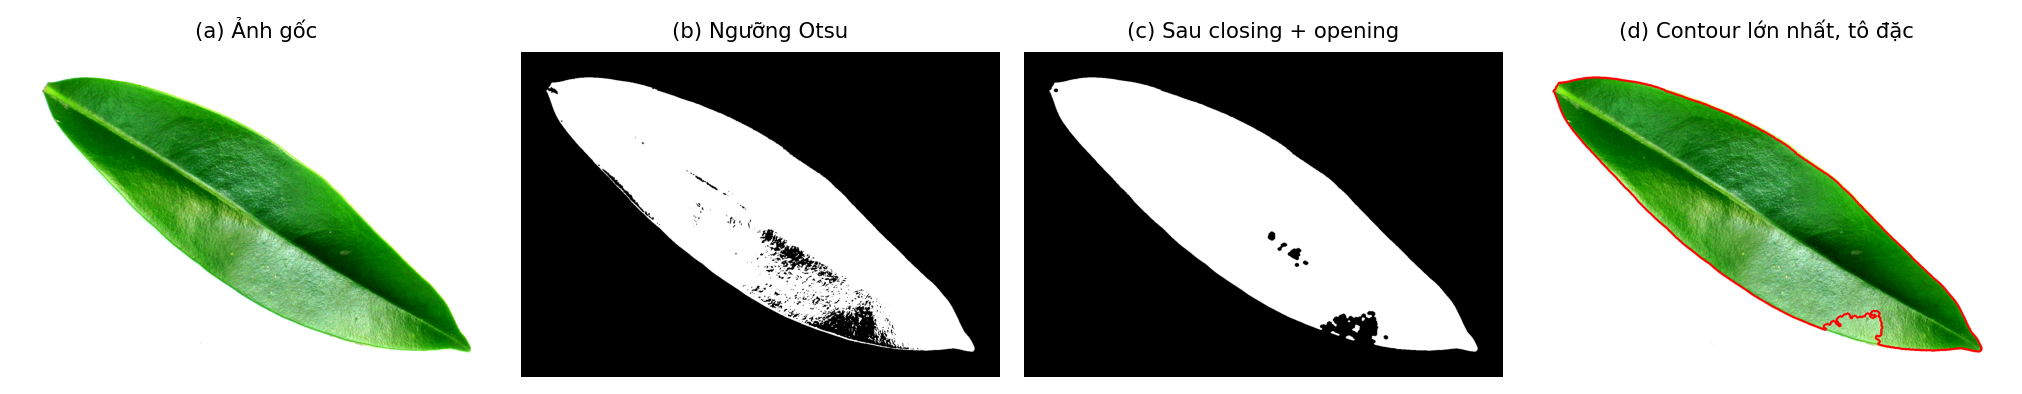
\includegraphics[width=\linewidth]{segmentation.png}
  \caption{Các bước phân đoạn trên một mẫu \emph{Ford Woodlotus} (ảnh 3267). Ảnh này được chọn vì
  bước hình thái học có tác dụng rõ rệt: mặt dưới lá nhạt màu bị ngưỡng Otsu (b) xếp nhầm vào nền,
  tạo một vùng thủng lớn, và phép đóng đã lấp gần hết vùng này (c). Với một lá điển hình, (b) và (c)
  gần như không khác nhau: các phép hình thái học chỉ thay đổi trung vị khoảng 1500 điểm ảnh, so với
  21000 điểm ảnh ở ảnh này. Phần thủng còn sót lại khiến đường viền (d) lõm nhẹ ở mép dưới; ảnh hưởng
  là nhỏ (solidity 0{,}973 so với trung vị 0{,}968 của toàn tập) nhưng phản ánh hạn chế của phương
  pháp ngưỡng toàn cục. Mép lá vẫn giữ nguyên độ chi tiết, là thông tin mà đặc trưng \emph{smooth
  factor} khai thác; do đó không thể tăng kích thước phần tử cấu trúc để loại bỏ phần còn sót.}
  \label{fig:segmentation}
\end{figure}

\subsection{Nhóm 1: đặc trưng hình dạng (\shapedims{} chiều)}
\label{sec:shape}

Nhóm này dựa trên tập đặc trưng hình học của Wu và cộng sự~\cite{wu2007}. Điểm khác biệt trong cài
đặt là chỉ giữ lại các đại lượng không thứ nguyên: diện tích hay chu vi tuyệt đối phụ thuộc vào
khoảng cách chụp chứ không phản ánh loài, và nếu được đưa vào, mô hình có thể học theo điều kiện
chụp thay vì hình thái lá.

Gọi $A$ là diện tích, $P$ là chu vi, $L$ và $W$ là chiều dài và chiều rộng sinh lý (các cạnh của hình
chữ nhật bao có diện tích nhỏ nhất), $D$ là đường kính của đường tròn bao nhỏ nhất. Các đặc trưng gồm:
\begin{align*}
\text{form factor} &= \frac{4\pi A}{P^2} & \text{rectangularity} &= \frac{LW}{A} \\
\text{aspect ratio} &= \frac{L}{W} & \text{solidity} &= \frac{A}{A_{\text{convex hull}}}
\end{align*}
cùng với hệ số hẹp $D/L$, các tỉ lệ chu vi $P/D$ và $P/(L{+}W)$, độ phủ (\emph{extent}), độ lệch tâm
của ellipse khớp, và \emph{smooth factor}, tức tỉ lệ chu vi còn lại sau khi làm mượt mặt nạ. Đặc
trưng này mô tả độ răng cưa của mép lá, vì mép răng cưa mất nhiều chu vi hơn mép trơn khi được làm
mượt. Khác với các đặc trưng còn lại trong nhóm, smooth factor sử dụng cửa sổ làm mượt có kích thước
cố định nên không bất biến theo tỉ lệ; hệ quả của điều này được đo ở mục~\ref{sec:invariance}.

Ngoài ra, nhóm hình dạng bao gồm bảy moment bất biến Hu~\cite{hu1962}, được biến đổi theo
$-\mathrm{sign}(h)\log_{10}|h|$. Các moment này bất biến với phép tịnh tiến, phép xoay và phép co
giãn, nhưng có miền giá trị chênh lệch nhiều bậc độ lớn; phép biến đổi logarit giúp bước chuẩn hoá
xử lý được chúng.

\subsection{Nhóm 2: đặc trưng màu sắc (\colordims{} chiều)}
\label{sec:color}

Nhóm này gồm ba moment màu (trung bình, độ lệch chuẩn và moment bậc ba) cho từng kênh trong hai
không gian màu RGB và HSV. Có hai lựa chọn cài đặt đáng lưu ý. Thứ nhất, các thống kê chỉ được tính
trên các điểm ảnh thuộc mặt nạ; nếu tính trên toàn ảnh, nền trắng sẽ chiếm đa số và làm mất khả năng
phân biệt của đặc trưng. Thứ hai, moment bậc ba được lấy căn bậc ba (giữ dấu) theo định nghĩa của
Stricker và Orengo~\cite{stricker1995}, để có cùng đơn vị với giá trị kênh màu. Không gian HSV được
sử dụng song song với RGB vì kênh sắc độ (Hue) giúp phân biệt các loài khác nhau về màu, và được cho
là ổn định hơn RGB khi độ sáng thay đổi; giả định này được kiểm chứng ở mục~\ref{sec:invariance}.

\subsection{Nhóm 3: đặc trưng kết cấu (\texturedims{} chiều)}
\label{sec:texture}

Đây là phần bổ sung so với Wu và cộng sự, theo hướng tiếp cận của Kadir và cộng sự~\cite{kadir2011}.

\textbf{Ma trận đồng xuất hiện mức xám (GLCM).} GLCM~\cite{haralick1973} đếm số cặp điểm ảnh có mức
xám $(i,j)$ cách nhau một vectơ dịch chuyển cho trước. Từ ma trận đã chuẩn hoá $p(i,j)$, các đại
lượng Haralick được tính như sau:
\[
\text{contrast} = \sum_{i,j} (i-j)^2 p(i,j), \qquad
\text{energy} = \sum_{i,j} p(i,j)^2, \qquad
\text{homogeneity} = \sum_{i,j} \frac{p(i,j)}{1+|i-j|}.
\]
Ảnh được lượng tử hoá về 32 mức xám, vì một ma trận $256\times256$ trên vài chục nghìn điểm ảnh sẽ
gần như toàn giá trị 0, làm các đại lượng correlation và energy mất ổn định về số học. Ma trận được
tính với hai khoảng cách $\{1,3\}$ và bốn hướng $\{0^\circ,45^\circ,90^\circ,135^\circ\}$, sau đó lấy
trung bình theo hướng nhằm làm đặc trưng bất biến với hướng đặt lá; mục~\ref{sec:invariance} cho thấy
tính bất biến này chỉ đúng với phép xoay là bội số của $90^\circ$. Mức xám 0 (nền) được loại khỏi
ma trận để các cặp điểm ảnh nằm vắt qua biên lá không ảnh hưởng đến thống kê.

\textbf{Mẫu nhị phân cục bộ (LBP).} LBP~\cite{ojala2002} so sánh mỗi điểm ảnh với 8 điểm lân cận trên
đường tròn bán kính 1 để tạo một mã nhị phân. Biến thể \emph{uniform} gộp các mã có nhiều hơn hai lần
chuyển bit vào cùng một nhóm, tạo thành histogram 10 chiều mô tả vi cấu trúc bề mặt lá.

\subsection{Nhóm 4: đặc trưng gân lá (\veindims{} chiều)}

Theo Wu và cộng sự~\cite{wu2007}, phép mở hình thái học với phần tử cấu trúc hình đĩa bán kính $r$
loại bỏ các cấu trúc mảnh hơn $r$; do đó hiệu giữa ảnh gốc và ảnh sau phép mở biểu diễn hệ gân. Với
$r = 1,2,3,4$, ảnh hiệu được nhị phân hoá bằng phương pháp Otsu để thu được diện tích gân $A_{v_r}$.
Đặc trưng là các tỉ lệ $A_{v_r}/A$ và $A_{v_r}/A_{v_1}$, vì diện tích tuyệt đối phụ thuộc vào tỉ lệ
ảnh. Bước nhị phân hoá này được phân tích chi tiết ở mục~\ref{sec:veinvariants}.

\section{Các bộ phân lớp và cơ sở lý thuyết}

Bốn bộ phân lớp được so sánh trên cùng một ma trận đặc trưng.

\textbf{SVM với nhân RBF.} Máy vectơ hỗ trợ~\cite{cortes1995} tìm siêu phẳng phân tách có lề cực đại.
Bài toán đối ngẫu chỉ phụ thuộc vào tích vô hướng giữa các mẫu, nên có thể thay tích vô hướng bằng
hàm nhân $K(x,x') = \exp(-\gamma\|x-x'\|^2)$ (\emph{kernel trick}), tương đương với việc ánh xạ dữ
liệu sang một không gian vô hạn chiều mà không cần tính tường minh phép ánh xạ. Hai tính chất này phù
hợp với bài toán đang xét: số chiều lớn (\bestdims{}--\totaldims{} chiều), số mẫu ít (1907), và tiêu
chí lề cực đại đóng vai trò như một cơ chế điều chuẩn hình học.

\textbf{KNN ($k=5$).} Phân lớp theo đa số trong 5 láng giềng gần nhất; phương pháp này nhạy với thang
đo và với hiện tượng ``lời nguyền số chiều'', theo đó khoảng cách giữa các điểm có xu hướng xấp xỉ
nhau khi số chiều tăng. \textbf{Random Forest (300 cây)~\cite{breiman2001}.} Bất biến với thang đo của
từng đặc trưng và mô hình hoá tốt các tương tác phi tuyến. \textbf{Gaussian Naive Bayes.} Giả định các
đặc trưng độc lập có điều kiện theo lớp; giả định này bị vi phạm đáng kể trong bài toán này (như được
đo ở mục~\ref{sec:redundancy}), vì vậy nó được dùng như cận dưới để so sánh.

\section{Thiết lập thực nghiệm}

\begin{itemize}
  \item \textbf{Đánh giá:} kiểm định chéo phân tầng 5 phần trên toàn bộ 1907 mẫu; kết quả báo cáo là
        trung bình và độ lệch chuẩn giữa các phần.
  \item \textbf{Chuẩn hoá:} mọi mô hình đều sử dụng chuẩn hoá z-score để bảo đảm so sánh công bằng.
  \item \textbf{Tránh rò rỉ dữ liệu:} bộ chuẩn hoá được đặt bên trong quy trình huấn luyện nên chỉ
        được ước lượng trên phần huấn luyện của mỗi lần chia. Nếu ước lượng trên toàn bộ dữ liệu,
        thống kê của tập kiểm tra sẽ rò rỉ vào quá trình huấn luyện và làm độ chính xác bị đánh giá
        cao hơn thực tế, ảnh hưởng trực tiếp đến các phép so sánh trong báo cáo.
  \item \textbf{Ablation:} toàn bộ 8 tổ hợp có chứa nhóm hình dạng (cấu hình cơ sở của Wu và cộng sự)
        kết hợp với 4 bộ phân lớp, tổng cộng 32 cấu hình.
  \item \textbf{Công cụ:} các bộ phân lớp và phép đánh giá được cài đặt bằng thư viện
        scikit-learn~\cite{pedregosa2011}.
\end{itemize}

\section{Kết quả và phân tích}
\label{sec:results}

Bảng~\ref{tab:ablation} và Hình~\ref{fig:ablation} trình bày toàn bộ kết quả ablation. Cấu hình tốt
nhất là \bestmodel{} trên nhóm \emph{\bestfeatures{}} (\bestdims{} chiều), đạt độ chính xác
\bestacc{} theo kiểm định chéo; trên tập kiểm tra giữ lại độc lập (25\% dữ liệu), mô hình này đạt
\holdoutacc{} (\holdouterrors{}/\holdouttotal{} mẫu bị phân lớp sai).

\begin{table}[t]
\centering
\caption{Độ chính xác trung bình theo kiểm định chéo phân tầng 5 phần trên Flavia (1907 ảnh, 32 loài). Giá trị in đậm là kết quả cao nhất của toàn bảng.}
\label{tab:ablation}
\small
\begin{tabular}{l r r r r r}
\toprule
Nhóm đặc trưng & \#chiều & KNN (k=5) & Naive Bayes & Random Forest & SVM (RBF) \\
\midrule
Hình dạng (cấu hình cơ sở) & 17 & 0{,}7897 & 0{,}8254 & 0{,}9025 & 0{,}8626 \\
Hình dạng + Màu & 35 & 0{,}9203 & 0{,}9554 & 0{,}9759 & 0{,}9759 \\
Hình dạng + Kết cấu & 39 & 0{,}9271 & 0{,}9313 & 0{,}9764 & 0{,}9790 \\
Hình dạng + Gân lá & 24 & 0{,}8180 & 0{,}8794 & 0{,}9554 & 0{,}9245 \\
Hình dạng + Màu + Kết cấu & 57 & 0{,}9554 & 0{,}9607 & 0{,}9843 & \textbf{0{,}9885} \\
Hình dạng + Màu + Gân lá & 42 & 0{,}9219 & 0{,}9575 & 0{,}9832 & 0{,}9780 \\
Hình dạng + Kết cấu + Gân lá & 46 & 0{,}9234 & 0{,}9428 & 0{,}9806 & 0{,}9754 \\
Tất cả bốn nhóm & 64 & 0{,}9586 & 0{,}9623 & 0{,}9858 & 0{,}9879 \\
\bottomrule
\end{tabular}
\end{table}

\begin{table}[t]
\centering
\caption{Toàn bộ mẫu bị phân lớp sai trên tập held-out 25\%.}
\label{tab:errors}
\small
\begin{tabular}{l l r}
\toprule
Nhãn thật & Dự đoán & Số mẫu \\
\midrule
Big-fruited Holly & wintersweet & 1 \\
Ford Woodlotus & southern magnolia & 1 \\
peach & camphortree & 1 \\
true indigo & Glossy Privet & 1 \\
wintersweet & Beale's barberry & 1 \\
\bottomrule
\end{tabular}
\end{table}

\begin{table}[t]
\centering
\caption{Ba phương pháp trích xuất gân lá, cùng ghép với nhóm \emph{Hình dạng + Màu + Kết cấu} và đánh giá trên cùng các phần kiểm định chéo. Không ô nào khác biệt có ý nghĩa thống kê so với dòng đầu (kiểm định $t$ ghép cặp; giá trị $p$ nhỏ nhất là 0{,}059 $> 0{,}05$).}
\label{tab:vein}
\small
\begin{tabular}{l r r r r}
\toprule
Cách trích xuất gân lá & KNN (k=5) & Naive Bayes & Random Forest & SVM (RBF) \\
\midrule
Không dùng gân lá & 0{,}9554 & 0{,}9607 & 0{,}9843 & 0{,}9885 \\
Ngưỡng Otsu (cách làm gốc) & 0{,}9586 & 0{,}9623 & 0{,}9858 & 0{,}9879 \\
Ngưỡng cố định tương đối & 0{,}9643 & 0{,}9654 & 0{,}9869 & 0{,}9895 \\
Bộ lọc Frangi & 0{,}9628 & 0{,}9696 & 0{,}9874 & 0{,}9879 \\
\bottomrule
\end{tabular}
\end{table}


\begin{figure}[t]
  \centering
  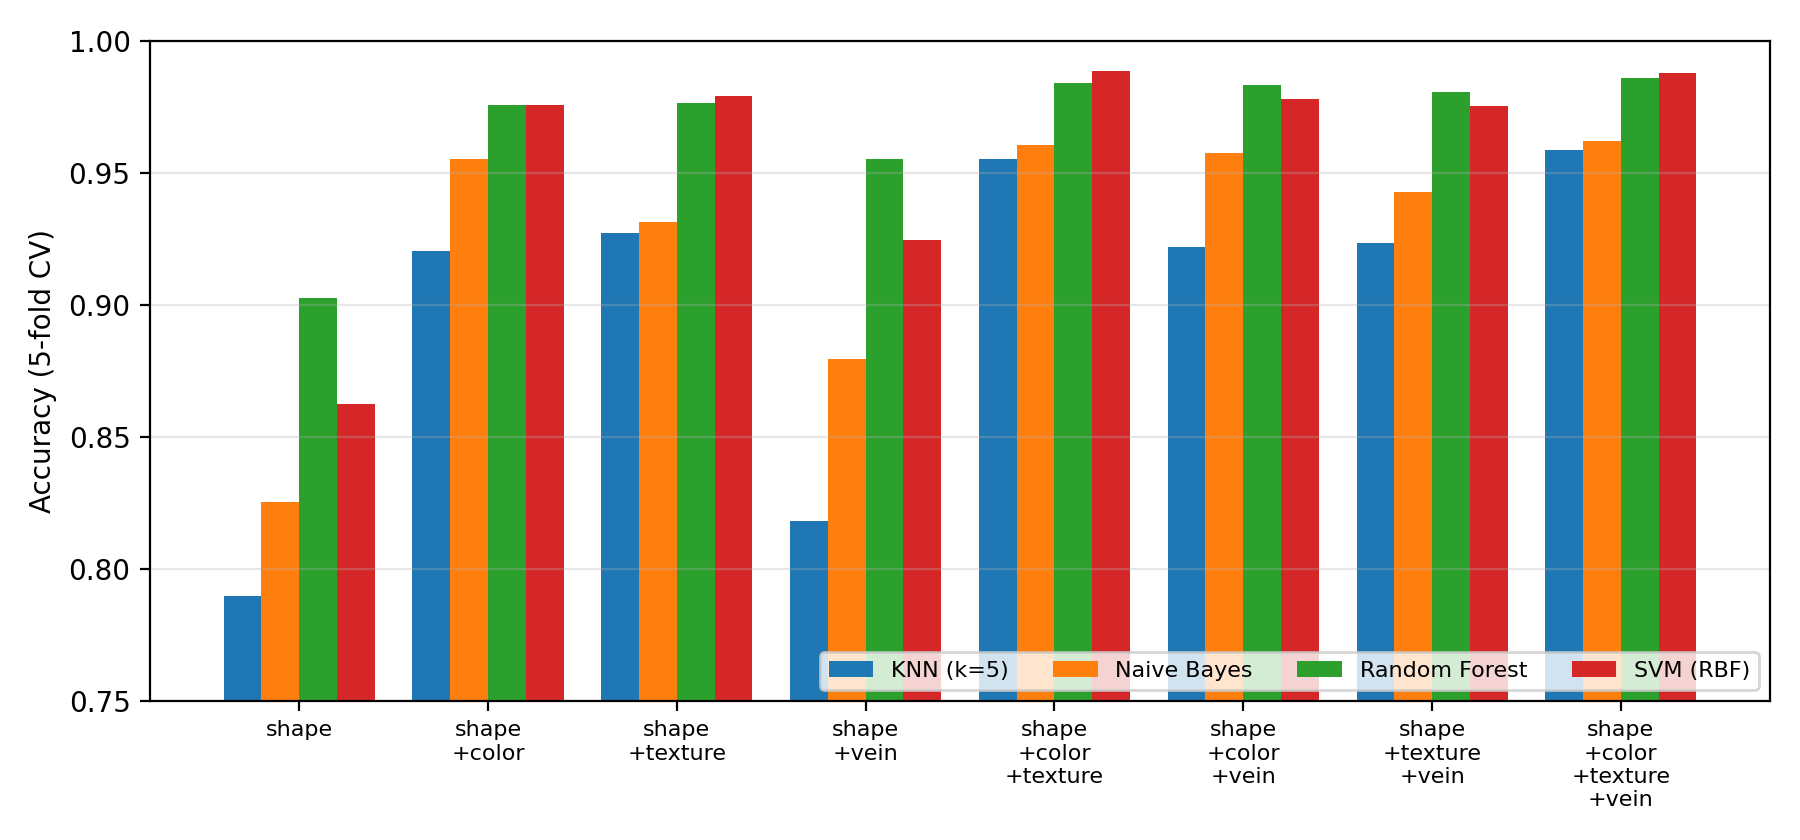
\includegraphics[width=\linewidth]{ablation.png}
  \caption{Độ chính xác theo tổ hợp nhóm đặc trưng và bộ phân lớp. Trục tung bắt đầu từ 0{,}75 để
  làm rõ khác biệt giữa các cấu hình.}
  \label{fig:ablation}
\end{figure}

\subsection{Đóng góp của nhóm màu sắc và nhóm kết cấu}

Với SVM, việc bổ sung nhóm màu vào cấu hình cơ sở chỉ gồm hình dạng làm độ chính xác tăng
\colorgain{} (từ \shapeonlyacc{} lên \shapecoloracc{}), trong khi bổ sung nhóm kết cấu vào tổ hợp
hình dạng và màu chỉ tăng thêm \texturegain{}. Điều này gợi ý rằng hai nhóm màu và kết cấu chồng lấn
thông tin đáng kể: khi được thêm riêng rẽ vào nhóm hình dạng, mỗi nhóm cho kết quả tương đương nhau,
nhưng khi kết hợp cả hai thì lợi ích không cộng dồn. Một cách giải thích hợp lý là cả hai nhóm đều
được tính trên vùng bên trong lá và cùng phản ánh tính chất bề mặt: lá bóng và sẫm màu khác lá mờ và
nhạt màu đồng thời cả về moment màu lẫn về độ tương phản GLCM. Nói cách khác, hai nhóm đo hai khía
cạnh của cùng một thuộc tính vật lý.

\subsubsection*{Kiểm chứng trực tiếp mức độ chồng lấn}
\label{sec:redundancy}

Lập luận trên suy ra mức độ chồng lấn một cách gián tiếp từ độ chính xác, trong khi độ chính xác là
một thước đo thô đối với lượng thông tin dùng chung. Vì vậy, mức độ chồng lấn được đo trực tiếp trên
ma trận đặc trưng:
\begin{itemize}
  \item \textbf{Phân tích tương quan chính tắc (CCA)~\cite{hotelling1936}.} Cặp màu--kết cấu có hệ số
        tương quan chính tắc thứ nhất $\rho_1 = \ccacolortexture{}$, cao hơn cặp kết cấu--hình dạng
        ($\ccatextureshape{}$) và cặp màu--hình dạng ($\ccacolorshape{}$). Như vậy, tồn tại một phép
        chiếu tuyến tính của khối đặc trưng màu gần như trùng khớp với một phép chiếu của khối kết cấu.
  \item \textbf{Hồi quy ridge.} Khi dự đoán từng đặc trưng kết cấu từ toàn bộ khối màu, hệ số xác định
        trung vị trên tập kiểm tra là $R^2 = \rtwocolortexture{}$ (và \rtwotexturecolor{} theo chiều
        ngược lại); nghĩa là gần một nửa phương sai của nhóm này đã được biểu diễn trong nhóm kia.
\end{itemize}

Hai phép đo này xác nhận kết luận rút ra từ độ chính xác, đồng thời giải thích vì sao việc kết hợp
hai nhóm chỉ đem lại thêm \texturegain{}: phần thông tin mới thực sự chỉ là phần còn lại sau khi đã
loại bỏ những gì hai nhóm cùng biểu diễn.

Một kết quả đáng lưu ý xuất hiện khi xét thông tin tương hỗ (\emph{mutual information}, MI) giữa từng
đặc trưng và nhãn: nhóm hình dạng có MI trung bình cao nhất (\mishape{}, so với \mitexture{} của nhóm
kết cấu và \micolor{} của nhóm màu), dù khi dùng riêng chỉ đạt \shapeonlyacc{}. Điều này không mâu
thuẫn: MI đo lượng thông tin mà từng đặc trưng mang về nhãn, còn độ chính xác phụ thuộc vào việc các
lớp có tách được trong không gian đặc trưng hay không. Đặc trưng hình dạng mang nhiều thông tin về loài,
nhưng 32 lớp vẫn chồng lấn đáng kể trong \shapedims{} chiều này; ngược lại, màu sắc và kết cấu tuy
mang ít thông tin hơn trên mỗi chiều nhưng làm tăng khoảng cách giữa các lớp. Độ quan trọng hoán vị
(\emph{permutation importance})~\cite{breiman2001} trên mô hình tốt nhất cũng xếp nhóm hình dạng cao
nhất (\impshape{}, với đặc trưng quan trọng nhất là smooth factor), tiếp theo là nhóm màu
(\impcolor{}) và nhóm kết cấu (\imptexture{}).

\textbf{Giới hạn của các phép chiếu hai chiều.} Hình~\ref{fig:projection} chiếu không gian đặc trưng
xuống hai chiều bằng PCA (không sử dụng nhãn) và LDA~\cite{fisher1936} (sử dụng nhãn để tìm các hướng
phân tách lớp). PCA hai chiều chỉ giữ lại \pcavarshape{}\% phương sai với nhóm hình dạng và
\pcavarbest{}\% với tổ hợp đầy đủ, do đó các lớp có vẻ chồng lấn nhiều dù SVM phân tách được chúng với
độ chính xác \bestacc{}. LDA cho kết quả tốt hơn, song hai hình LDA gần như giống nhau: với cả hai tập
đặc trưng, hai trục phân biệt đầu tiên đều dành cho ba loài có hình dạng khác biệt nhất
(\ldaoutliers{}). Phép đo bằng KNN trên $k$ trục LDA đầu tiên (LDA được ước lượng lại trong mỗi lần
chia) xác nhận điều này: với 2 trục, nhóm hình dạng đạt \ldaknnshapetwo{} và tổ hợp đầy đủ đạt
\ldaknnbesttwo{}, gần như không khác biệt; với 10 trục, hai con số lần lượt là \ldaknnshapeten{} và
\ldaknnbestten{}. Như vậy, lợi ích của màu sắc và kết cấu là có thật nhưng nằm ở các chiều sau chiều
thứ hai, nên không phép chiếu hai chiều nào thể hiện được. Điều này cho thấy khả năng phân tách lớp
cần được đánh giá bằng số liệu định lượng thay vì chỉ bằng quan sát trực quan.

\begin{figure}[t]
  \centering
  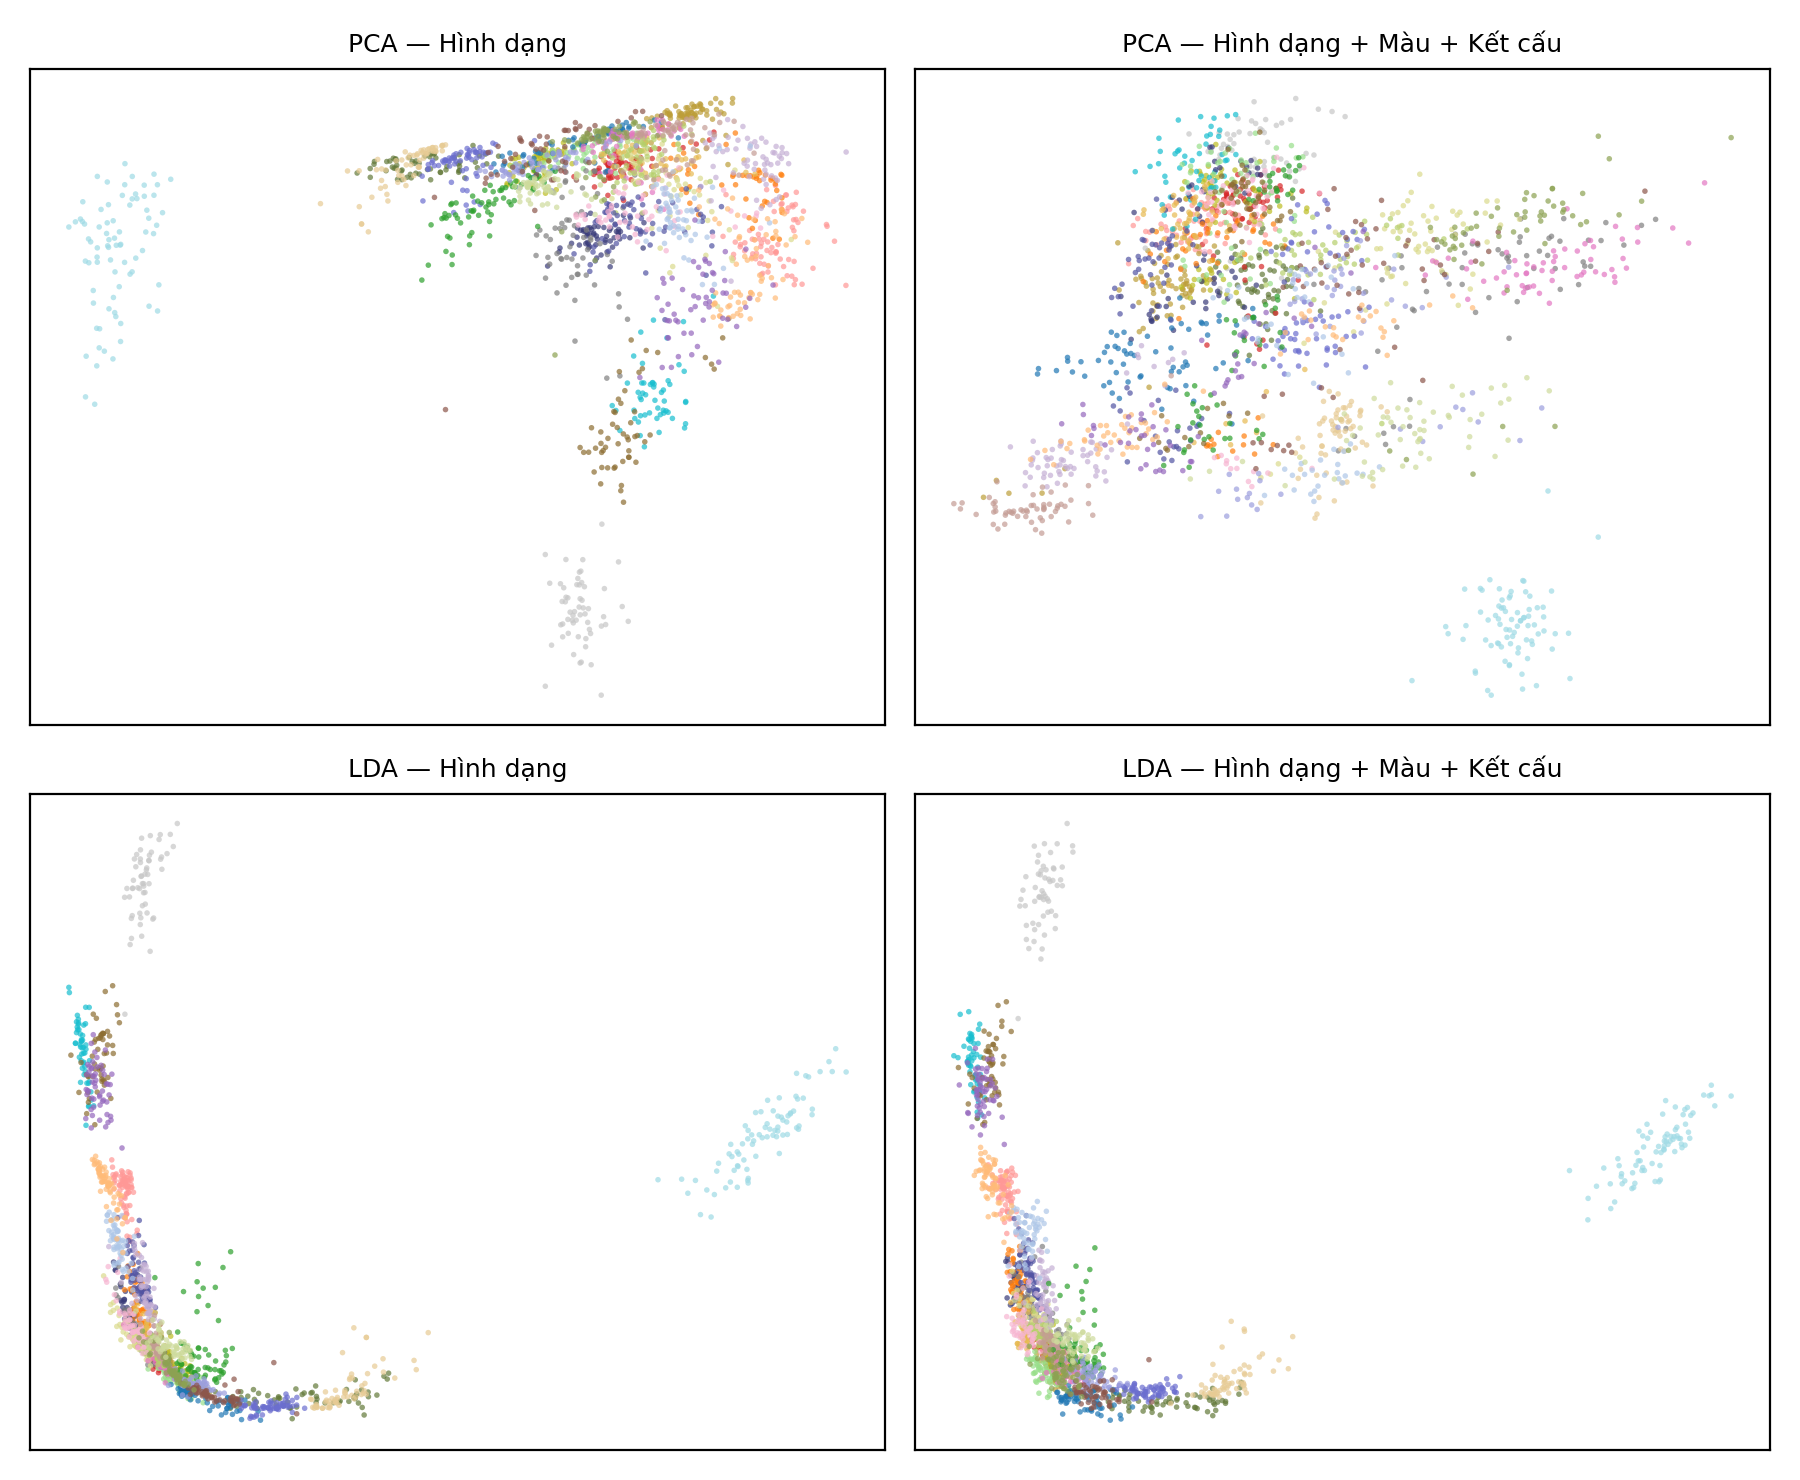
\includegraphics[width=0.92\linewidth]{projection.png}
  \caption{Không gian đặc trưng chiếu xuống hai chiều; mỗi màu tương ứng với một loài. Các phép chiếu
  được ước lượng trên toàn bộ dữ liệu nên chỉ mang tính minh hoạ; mọi giá trị độ chính xác trong văn
  bản đều lấy từ kiểm định chéo.}
  \label{fig:projection}
\end{figure}

\subsection{Đóng góp của nhóm gân lá}

Việc bổ sung nhóm gân lá vào tổ hợp tốt nhất làm độ chính xác của SVM thay đổi $\veinotsusvm$ điểm
phần trăm (từ \bestacc{} xuống \allgroupsacc{}). Kết quả này dễ bị diễn giải thành ``nhóm gân lá làm
giảm chất lượng mô hình'', tuy nhiên diễn giải đó không có cơ sở: độ lệch chuẩn giữa các phần kiểm
định của chính cấu hình tốt nhất là \beststd{} điểm phần trăm, lớn hơn gần mười lần mức chênh lệch nói
trên. Kiểm định $t$ ghép cặp trên từng phần cho $p = \veinotsusvmp{}$, tức không có bằng chứng thống kê
cho thấy nhóm gân lá làm thay đổi kết quả theo bất kỳ hướng nào.

Do đó, kết luận chính xác là nhóm gân lá trong cài đặt này không có đóng góp đo được, chứ không phải
có tác động tiêu cực. Mục~\ref{sec:veinvariants} phân tích nguyên nhân của kết quả này.

\subsection{Ảnh hưởng của phương pháp nhị phân hoá gân lá}
\label{sec:veinvariants}

Kết quả ở mục trước là nhận định về cách cài đặt cụ thể, không phải về đặc trưng gân lá nói chung.
Giả thuyết được đặt ra là bước nhị phân hoá ảnh hiệu bằng phương pháp Otsu: do Otsu luôn chia
histogram thành hai lớp, với những lá có gân mờ (khi ảnh hiệu chủ yếu chứa nhiễu), phương pháp này
vẫn trả về một ngưỡng và tạo ra ``diện tích gân'' thực chất là nhiễu.

Để kiểm chứng giả thuyết, bước này được thay thế bằng hai phương án, trong khi các thành phần khác được
giữ nguyên:
\begin{itemize}
  \item \textbf{Ngưỡng cố định tương đối:} ngưỡng bằng $0{,}3 \times P_{99}$ của ảnh hiệu bên trong lá.
        Khác với Otsu, phương án này có thể trả về diện tích bằng 0, là kết quả đúng đối với những lá
        mà phép mở không tách được gân.
  \item \textbf{Bộ lọc Frangi}~\cite{frangi1998}: bộ lọc được thiết kế cho các cấu trúc dạng ống, đánh
        giá mỗi điểm ảnh dựa trên các trị riêng của ma trận Hessian; bộ lọc cho đáp ứng mạnh tại những
        vị trí có độ cong lớn theo một hướng và gần như phẳng theo hướng còn lại, tương ứng với gân lá.
\end{itemize}

Kết quả được trình bày ở Bảng~\ref{tab:vein}. Với SVM, cả hai phương án đều không tạo ra khác biệt có
ý nghĩa thống kê ($\veinpctsvm$ điểm, $p = \veinpctsvmp{}$ với ngưỡng cố định; $\veinfrangisvm$ điểm,
$p = \veinfrangisvmp{}$ với bộ lọc Frangi). Tuy nhiên, có một xu hướng nhất quán: cả hai phương án mới
đều cho kết quả cao hơn Otsu với cả bốn bộ phân lớp, và mức cải thiện lớn nhất xuất hiện ở các bộ phân
lớp yếu hơn. Với KNN, ngưỡng cố định cải thiện $\veinpctknn$ điểm ($p = \veinpctknnp{}$) và bộ lọc
Frangi cải thiện $\veinfrangiknn$ điểm ($p = \veinfrangiknnp{}$), so với $\veinotsuknn$ điểm của Otsu.

Cách diễn giải nhất quán với toàn bộ số liệu là: thông tin về gân lá là có thật và Otsu là lựa chọn
chưa phù hợp cho bước nhị phân hoá, nhưng thông tin này phần lớn đã được biểu diễn trong nhóm màu và
nhóm kết cấu. Các bộ phân lớp mạnh (SVM, Random Forest) đã khai thác phần thông tin này thông qua các
nhóm khác, trong khi các bộ phân lớp yếu hơn vẫn tận dụng được một phần. Cần nhấn mạnh rằng không có
phép so sánh nào đạt mức ý nghĩa $p < 0{,}05$ với 5 phần kiểm định, nên đây mới là xu hướng chứ chưa
phải kết luận chắc chắn.

\subsection{Điều kiện để SVM đạt ưu thế}

Một kết quả đáng chú ý của Bảng~\ref{tab:ablation} là SVM dẫn đầu ở các tổ hợp có nhiều nhóm đặc
trưng, nhưng thua Random Forest một cách rõ rệt ở cấu hình chỉ có hình dạng (\shapeonlyacc{} so với
\shapeonlyrf{}).

Kết quả này phù hợp với lý thuyết. Trong không gian \shapedims{} chiều hình học, các lớp chồng lấn
nhiều và biên quyết định phụ thuộc vào tương tác giữa các đặc trưng (chẳng hạn aspect ratio nhỏ đồng
thời solidity cao). Cây quyết định biểu diễn trực tiếp dạng biên này bằng các phép chia theo trục,
trong khi nhân RBF phải xấp xỉ bằng tổ hợp các hàm Gauss. Khi bổ sung màu sắc và kết cấu, số chiều
tăng và các lớp trở nên dễ phân tách hơn; khi đó ưu thế của tiêu chí lề cực đại mới được phát huy.
Vì vậy, kết luận phù hợp không phải là ``SVM luôn tốt nhất'', mà là SVM đạt hiệu quả cao nhất trên
không gian đặc trưng nhiều chiều và có khả năng phân tách tốt, đúng như lý thuyết lề cực đại dự đoán.

\subsection{Phân tích lỗi}

Bảng~\ref{tab:errors} liệt kê toàn bộ \holdouterrors{} mẫu bị phân lớp sai trên tập kiểm tra giữ lại
(ma trận nhầm lẫn đầy đủ được trình bày ở Phụ lục, Hình~\ref{fig:confusion}). Mỗi cặp nhầm lẫn chỉ
xuất hiện một lần và không có cặp loài nào bị nhầm lặp lại, cho thấy mô hình không mắc lỗi mang tính
hệ thống mà chỉ sai ở một số mẫu nằm gần biên quyết định.

\todo{mở ảnh của vài mẫu sai trong Bảng~\ref{tab:errors} và nhận xét bằng quan sát trực quan:
các cặp này có giống nhau về hình dạng/màu không?}

\subsection{Kiểm chứng tính bất biến}
\label{sec:invariance}

Các mục trên chỉ đánh giá độ chính xác trên dữ liệu sạch. Trong khi đó, phần phương pháp dựa trên một
số giả định về tính bất biến: moment Hu bất biến với phép xoay và phép co giãn, việc lấy trung bình
GLCM theo bốn hướng tạo ra tính bất biến theo hướng, và không gian HSV ổn định hơn RGB khi độ sáng thay
đổi. Thực nghiệm này kiểm chứng các giả định đó: mô hình được huấn luyện trên ảnh sạch và được đánh giá
trên ảnh đã qua các phép biến đổi có kiểm soát, với từng nhóm đặc trưng được đánh giá riêng để xác
định nguyên nhân của mức suy giảm (Hình~\ref{fig:invariance}).

\textbf{Đối chứng.} Với phép biến đổi đồng nhất (\emph{identity}), độ chính xác đạt \invcontrol{},
trùng khớp với kết quả trên tập kiểm tra giữ lại ở mục~\ref{sec:results}. Điều kiện này bảo đảm quy
trình trích xuất lại đặc trưng là chính xác, và các mức suy giảm quan sát được là do phép biến đổi chứ
không phải do lỗi cài đặt.

\begin{figure}[t]
  \centering
  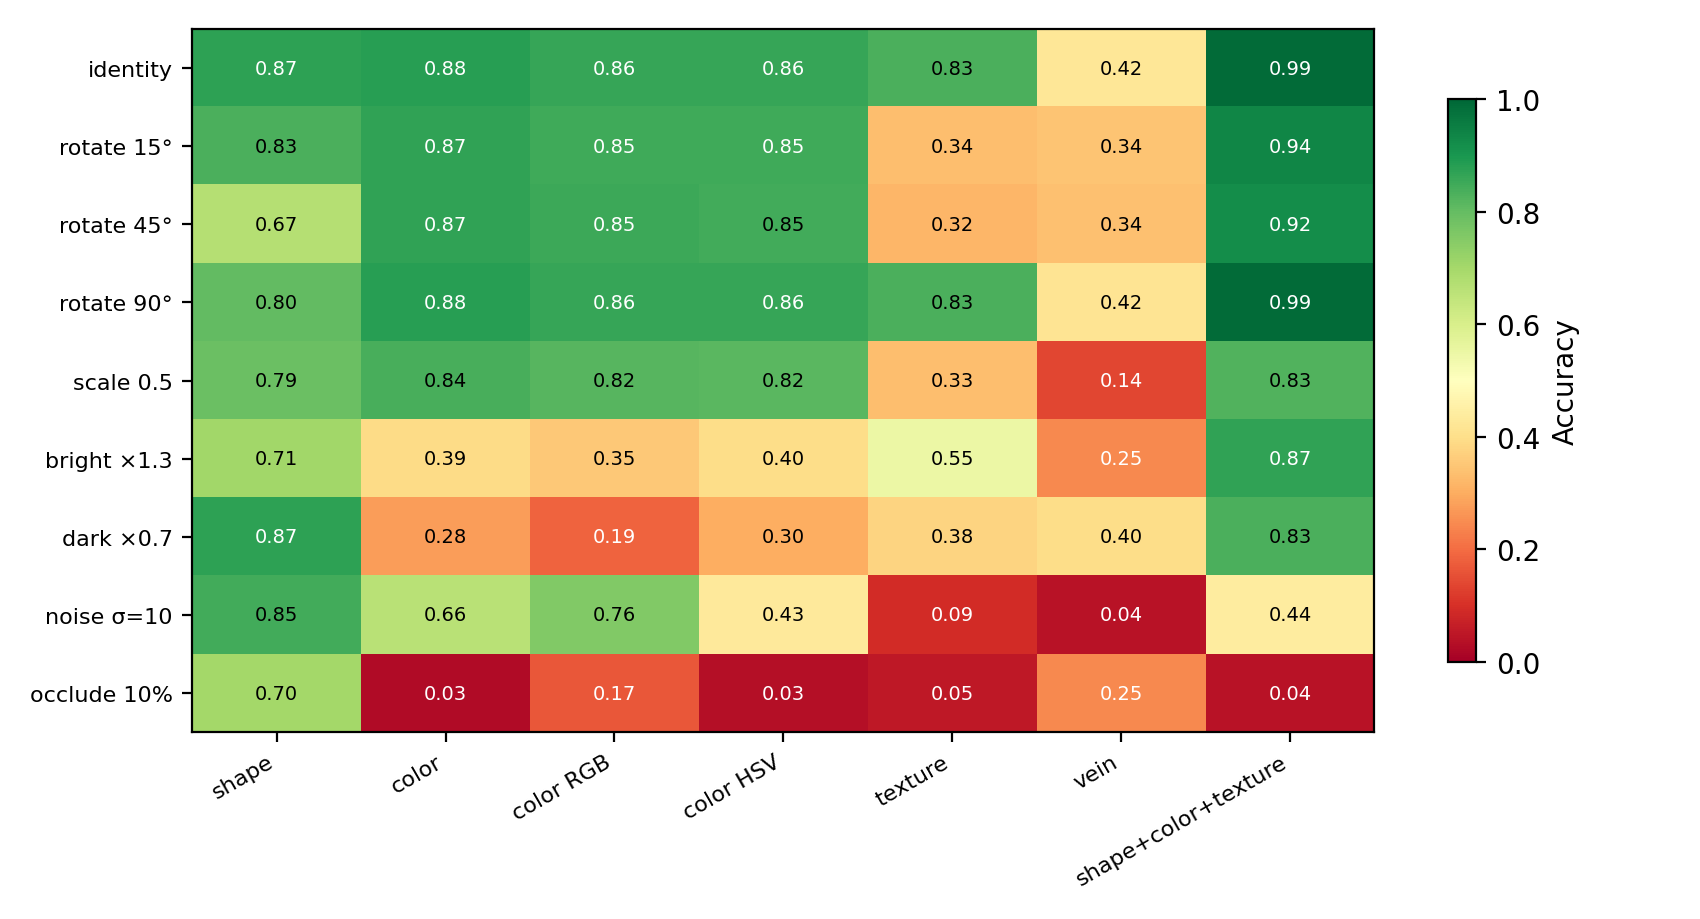
\includegraphics[width=\linewidth]{invariance.png}
  \caption{Độ chính xác khi huấn luyện trên ảnh sạch và kiểm tra trên ảnh đã biến đổi. Hàng
  \emph{identity} là phép đối chứng.}
  \label{fig:invariance}
\end{figure}

\textbf{Kết quả 1: đặc trưng kết cấu chỉ bất biến với phép xoay là bội số của $90^\circ$.} Độ chính xác
của nhóm kết cấu giữ nguyên \invtexrotninety{} khi xoay $90^\circ$ (bằng giá trị trên ảnh gốc), nhưng
giảm xuống \invtexrotfifteen{} khi chỉ xoay $15^\circ$. Mức dịch chuyển của từng đặc trưng (tính theo
đơn vị độ lệch chuẩn của chính đặc trưng đó) làm rõ cơ chế: ở $90^\circ$, GLCM dịch chuyển
\driftglcmninety{} và LBP dịch chuyển \driftlbpninety{}, tức gần như không đổi; ở $15^\circ$, các giá
trị tương ứng là \driftglcmfifteen{} và \driftlbpfifteen{}. Đáng lưu ý là mức dịch chuyển ở $45^\circ$
tương đương với ở $15^\circ$, mặc dù về lý thuyết tập hướng $\{0^\circ,45^\circ,90^\circ,135^\circ\}$
của GLCM được ánh xạ lên chính nó qua phép xoay $45^\circ$. Như vậy, nguyên nhân không nằm ở tập hướng
mà ở lưới điểm ảnh: mọi phép xoay không vuông góc đều đòi hỏi nội suy, và phép nội suy làm biến đổi
chính vi cấu trúc mà GLCM và LBP đo lường. Giả định về tính bất biến theo hướng ở mục~\ref{sec:texture}
do đó chỉ đúng với ảnh quét của Flavia (lá luôn được đặt thẳng) và không còn đúng với ảnh chụp tự do.

\textbf{Kết quả 2: đặc trưng quan trọng nhất cũng là đặc trưng kém bất biến nhất.} Độ chính xác của
nhóm hình dạng giảm từ \invshapeid{} xuống \invshaperotninety{} khi xoay $90^\circ$, mặc dù về mặt hình
học phép xoay này không làm thay đổi lá. Toàn bộ mức suy giảm này bắt nguồn từ một đặc trưng duy nhất:
smooth factor dịch chuyển \driftsmoothninety{} độ lệch chuẩn, trong khi mọi đặc trưng hình dạng khác
dịch chuyển dưới 0{,}05. Nguyên nhân là smooth factor được tính từ chu vi, và chu vi nhạy với hiện
tượng khử răng cưa tại biên sau khi nội suy. Kết quả này đáng chú ý vì phân tích độ quan trọng hoán vị
ở mục~\ref{sec:redundancy} cho thấy smooth factor là đặc trưng quan trọng nhất của mô hình.

Khi thu nhỏ ảnh còn một nửa, smooth factor dịch chuyển tới \driftsmoothscale{} độ lệch chuẩn, làm độ
chính xác của nhóm hình dạng giảm từ \invshapeid{} xuống \invshapescale{}. Đây là hạn chế trong thiết
kế của cài đặt hiện tại, không phải của phương pháp: smooth factor làm mượt mặt nạ bằng cửa sổ
$5\times5$ có kích thước cố định, nên khi kích thước lá giảm một nửa, độ răng cưa tương đối so với
cửa sổ cũng thay đổi. Để đạt tính bất biến theo tỉ lệ, kích thước cửa sổ cần tỉ lệ với chu vi lá.

\textbf{Kết quả 3: HSV ổn định hơn RGB, nhưng cả hai đều không bền vững.} Giả định ở
mục~\ref{sec:color} được số liệu ủng hộ về mặt xu hướng: khi giảm độ sáng, nhóm HSV đạt \invhsvdark{}
trong khi nhóm RGB chỉ đạt \invrgbdark{}. Tuy nhiên, cả hai đều suy giảm mạnh so với mức \invhsvid{}
trên ảnh gốc, nên phát biểu chính xác là ``HSV suy giảm chậm hơn RGB'' chứ không phải ``HSV ổn định''.
Ngược lại, khi ảnh bị nhiễu Gauss, RGB (\invrgbnoise{}) lại bền vững hơn HSV (\invhsvnoise{}), do kênh
sắc độ rất nhạy với nhiễu tại các điểm ảnh có độ bão hoà thấp.

\textbf{Kết quả 4: việc kết hợp đặc trưng làm giảm độ bền vững của mô hình.} Đây là kết quả trái với
kỳ vọng nhất. Khi ảnh bị nhiễu Gauss, nhóm hình dạng vẫn đạt \invshapenoise{} nhưng tổ hợp đầy đủ chỉ
còn \invcombonoise{}; khi bị che khuất 10\%, nhóm hình dạng đạt \invshapeoccl{} trong khi tổ hợp giảm
xuống \invcombooccl{}. Nói cách khác, tổ hợp tốt nhất trên dữ liệu sạch lại kém hơn đáng kể so với một
nhóm đặc trưng đơn lẻ khi dữ liệu bị nhiễu. Nguyên nhân là SVM được huấn luyện trên dữ liệu sạch đã
học trọng số cho toàn bộ \bestdims{} chiều và không có cơ chế bỏ qua những chiều bị sai lệch; các
chiều kết cấu bị nhiễu đẩy mẫu ra khỏi vùng quyết định đúng, bất kể các chiều hình dạng vẫn còn
nguyên vẹn. Điều này cho thấy độ chính xác \bestacc{} chỉ có giá trị trong đúng điều kiện thu nhận
ảnh của Flavia.

\section{Hạn chế}

\begin{itemize}
  \item Flavia được thu nhận trong điều kiện lý tưởng (nền trắng, mỗi ảnh một lá, đủ sáng). Phương pháp
        phân đoạn dựa trên ngưỡng Otsu toàn cục sẽ không còn phù hợp với ảnh chụp ngoài thực địa.
  \item Ngay trên Flavia, ngưỡng toàn cục đã cho lỗi cục bộ với các lá có mặt dưới nhạt màu
        (Hình~\ref{fig:segmentation}d); các phương pháp ngưỡng thích nghi hoặc GrabCut có thể xử lý
        tốt hơn.
  \item Các siêu tham số ($C$, $\gamma$, $k$, số cây) được cố định thay vì được lựa chọn bằng tìm kiếm
        lưới với kiểm định chéo lồng nhau.
  \item Với 5 phần kiểm định, các khác biệt nhỏ hơn khoảng 1 điểm phần trăm không đạt mức ý nghĩa
        thống kê (mục~\ref{sec:veinvariants}). Để có kết luận chắc chắn về nhóm gân lá, cần tăng số
        phần kiểm định hoặc lặp lại kiểm định nhiều lần.
\end{itemize}

\section{Kết luận}

Quy trình kết hợp đặc trưng thủ công với SVM đạt độ chính xác \bestacc{} trên 32 loài của Flavia, cao
hơn mức 93,75\% mà Kadir và cộng sự~\cite{kadir2011} báo cáo trên cùng bộ dữ liệu (dù giao thức đánh
giá không hoàn toàn giống nhau). Cấu hình cơ sở chỉ dùng hình dạng đạt \shapeonlyacc{}--\shapeonlyrf{},
tương đương mức trên 90\% của Wu và cộng sự~\cite{wu2007}; hai mốc so sánh này cho thấy cài đặt không
có sai lệch bất thường. Quan trọng hơn con số độ chính xác, thực nghiệm ablation cho thấy đóng góp của
các nhóm đặc trưng rất không đồng đều, và việc so sánh nhiều bộ phân lớp cho phép xác định cụ thể điều
kiện để SVM đạt ưu thế, thay vì chỉ khẳng định SVM là tốt nhất. Kết quả đối với nhóm gân lá cũng đem
lại một bài học về phương pháp luận: chênh lệch $\veinotsusvm$ điểm phần trăm thoạt nhìn giống một kết
quả âm, nhưng khi đặt cạnh độ lệch chuẩn giữa các phần kiểm định, nó chỉ là nhiễu; mọi khác biệt nhỏ
cần được kiểm định ghép cặp trước khi diễn giải.

Cuối cùng, thực nghiệm ở mục~\ref{sec:invariance} cho thấy độ chính xác \bestacc{} tuy đúng nhưng có
phạm vi áp dụng hẹp, chỉ có giá trị trong điều kiện thu nhận ảnh của Flavia. Chỉ cần xoay lá
$15^\circ$ hoặc thêm một mức nhiễu vừa phải, mô hình tốt nhất đã có độ chính xác thấp hơn nhóm hình
dạng đơn lẻ. Đối với một hệ thống ứng dụng thực tế, độ bền vững trước các phép biến đổi cần được xem
trọng ngang với độ chính xác trên tập kiểm tra sạch.

\begin{thebibliography}{99}

\bibitem{wu2007}
S.~G. Wu, F.~S. Bao, E.~Y. Xu, Y.-X. Wang, Y.-F. Chang, and Q.-L. Xiang, ``A leaf recognition
algorithm for plant classification using probabilistic neural network,'' in \emph{Proc. IEEE Int.
Symp. Signal Processing and Information Technology (ISSPIT)}, 2007, pp.~11--16.

\bibitem{kadir2011}
A.~Kadir, L.~E. Nugroho, A.~Susanto, and P.~I. Santosa, ``Leaf classification using shape, color,
and texture features,'' \emph{International Journal of Computer Trends and Technology}, vol.~1,
no.~3, pp.~306--311, 2011.

\bibitem{otsu1979}
N.~Otsu, ``A threshold selection method from gray-level histograms,'' \emph{IEEE Transactions on
Systems, Man, and Cybernetics}, vol.~9, no.~1, pp.~62--66, 1979.

\bibitem{hu1962}
M.-K. Hu, ``Visual pattern recognition by moment invariants,'' \emph{IRE Transactions on
Information Theory}, vol.~8, no.~2, pp.~179--187, 1962.

\bibitem{stricker1995}
M.~Stricker and M.~Orengo, ``Similarity of color images,'' in \emph{Proc. SPIE 2420, Storage and
Retrieval for Image and Video Databases III}, 1995, pp.~381--392.

\bibitem{haralick1973}
R.~M. Haralick, K.~Shanmugam, and I.~Dinstein, ``Textural features for image classification,''
\emph{IEEE Transactions on Systems, Man, and Cybernetics}, vol.~SMC-3, no.~6, pp.~610--621, 1973.

\bibitem{ojala2002}
T.~Ojala, M.~Pietikäinen, and T.~Mäenpää, ``Multiresolution gray-scale and rotation invariant
texture classification with local binary patterns,'' \emph{IEEE Transactions on Pattern Analysis
and Machine Intelligence}, vol.~24, no.~7, pp.~971--987, 2002.

\bibitem{cortes1995}
C.~Cortes and V.~Vapnik, ``Support-vector networks,'' \emph{Machine Learning}, vol.~20, no.~3,
pp.~273--297, 1995.

\bibitem{breiman2001}
L.~Breiman, ``Random forests,'' \emph{Machine Learning}, vol.~45, no.~1, pp.~5--32, 2001.

\bibitem{pedregosa2011}
F.~Pedregosa \emph{et al.}, ``Scikit-learn: Machine learning in Python,'' \emph{Journal of Machine
Learning Research}, vol.~12, pp.~2825--2830, 2011.

\bibitem{hotelling1936}
H.~Hotelling, ``Relations between two sets of variates,'' \emph{Biometrika}, vol.~28, no.~3/4,
pp.~321--377, 1936.

\bibitem{fisher1936}
R.~A. Fisher, ``The use of multiple measurements in taxonomic problems,'' \emph{Annals of
Eugenics}, vol.~7, no.~2, pp.~179--188, 1936.

\bibitem{frangi1998}
A.~F. Frangi, W.~J. Niessen, K.~L. Vincken, and M.~A. Viergever, ``Multiscale vessel enhancement
filtering,'' in \emph{Medical Image Computing and Computer-Assisted Intervention (MICCAI)}, Lecture
Notes in Computer Science, vol.~1496, 1998, pp.~130--137.

\end{thebibliography}

\appendix
\section*{Phụ lục}
\addcontentsline{toc}{section}{Phụ lục}

\begin{figure}[h]
  \centering
  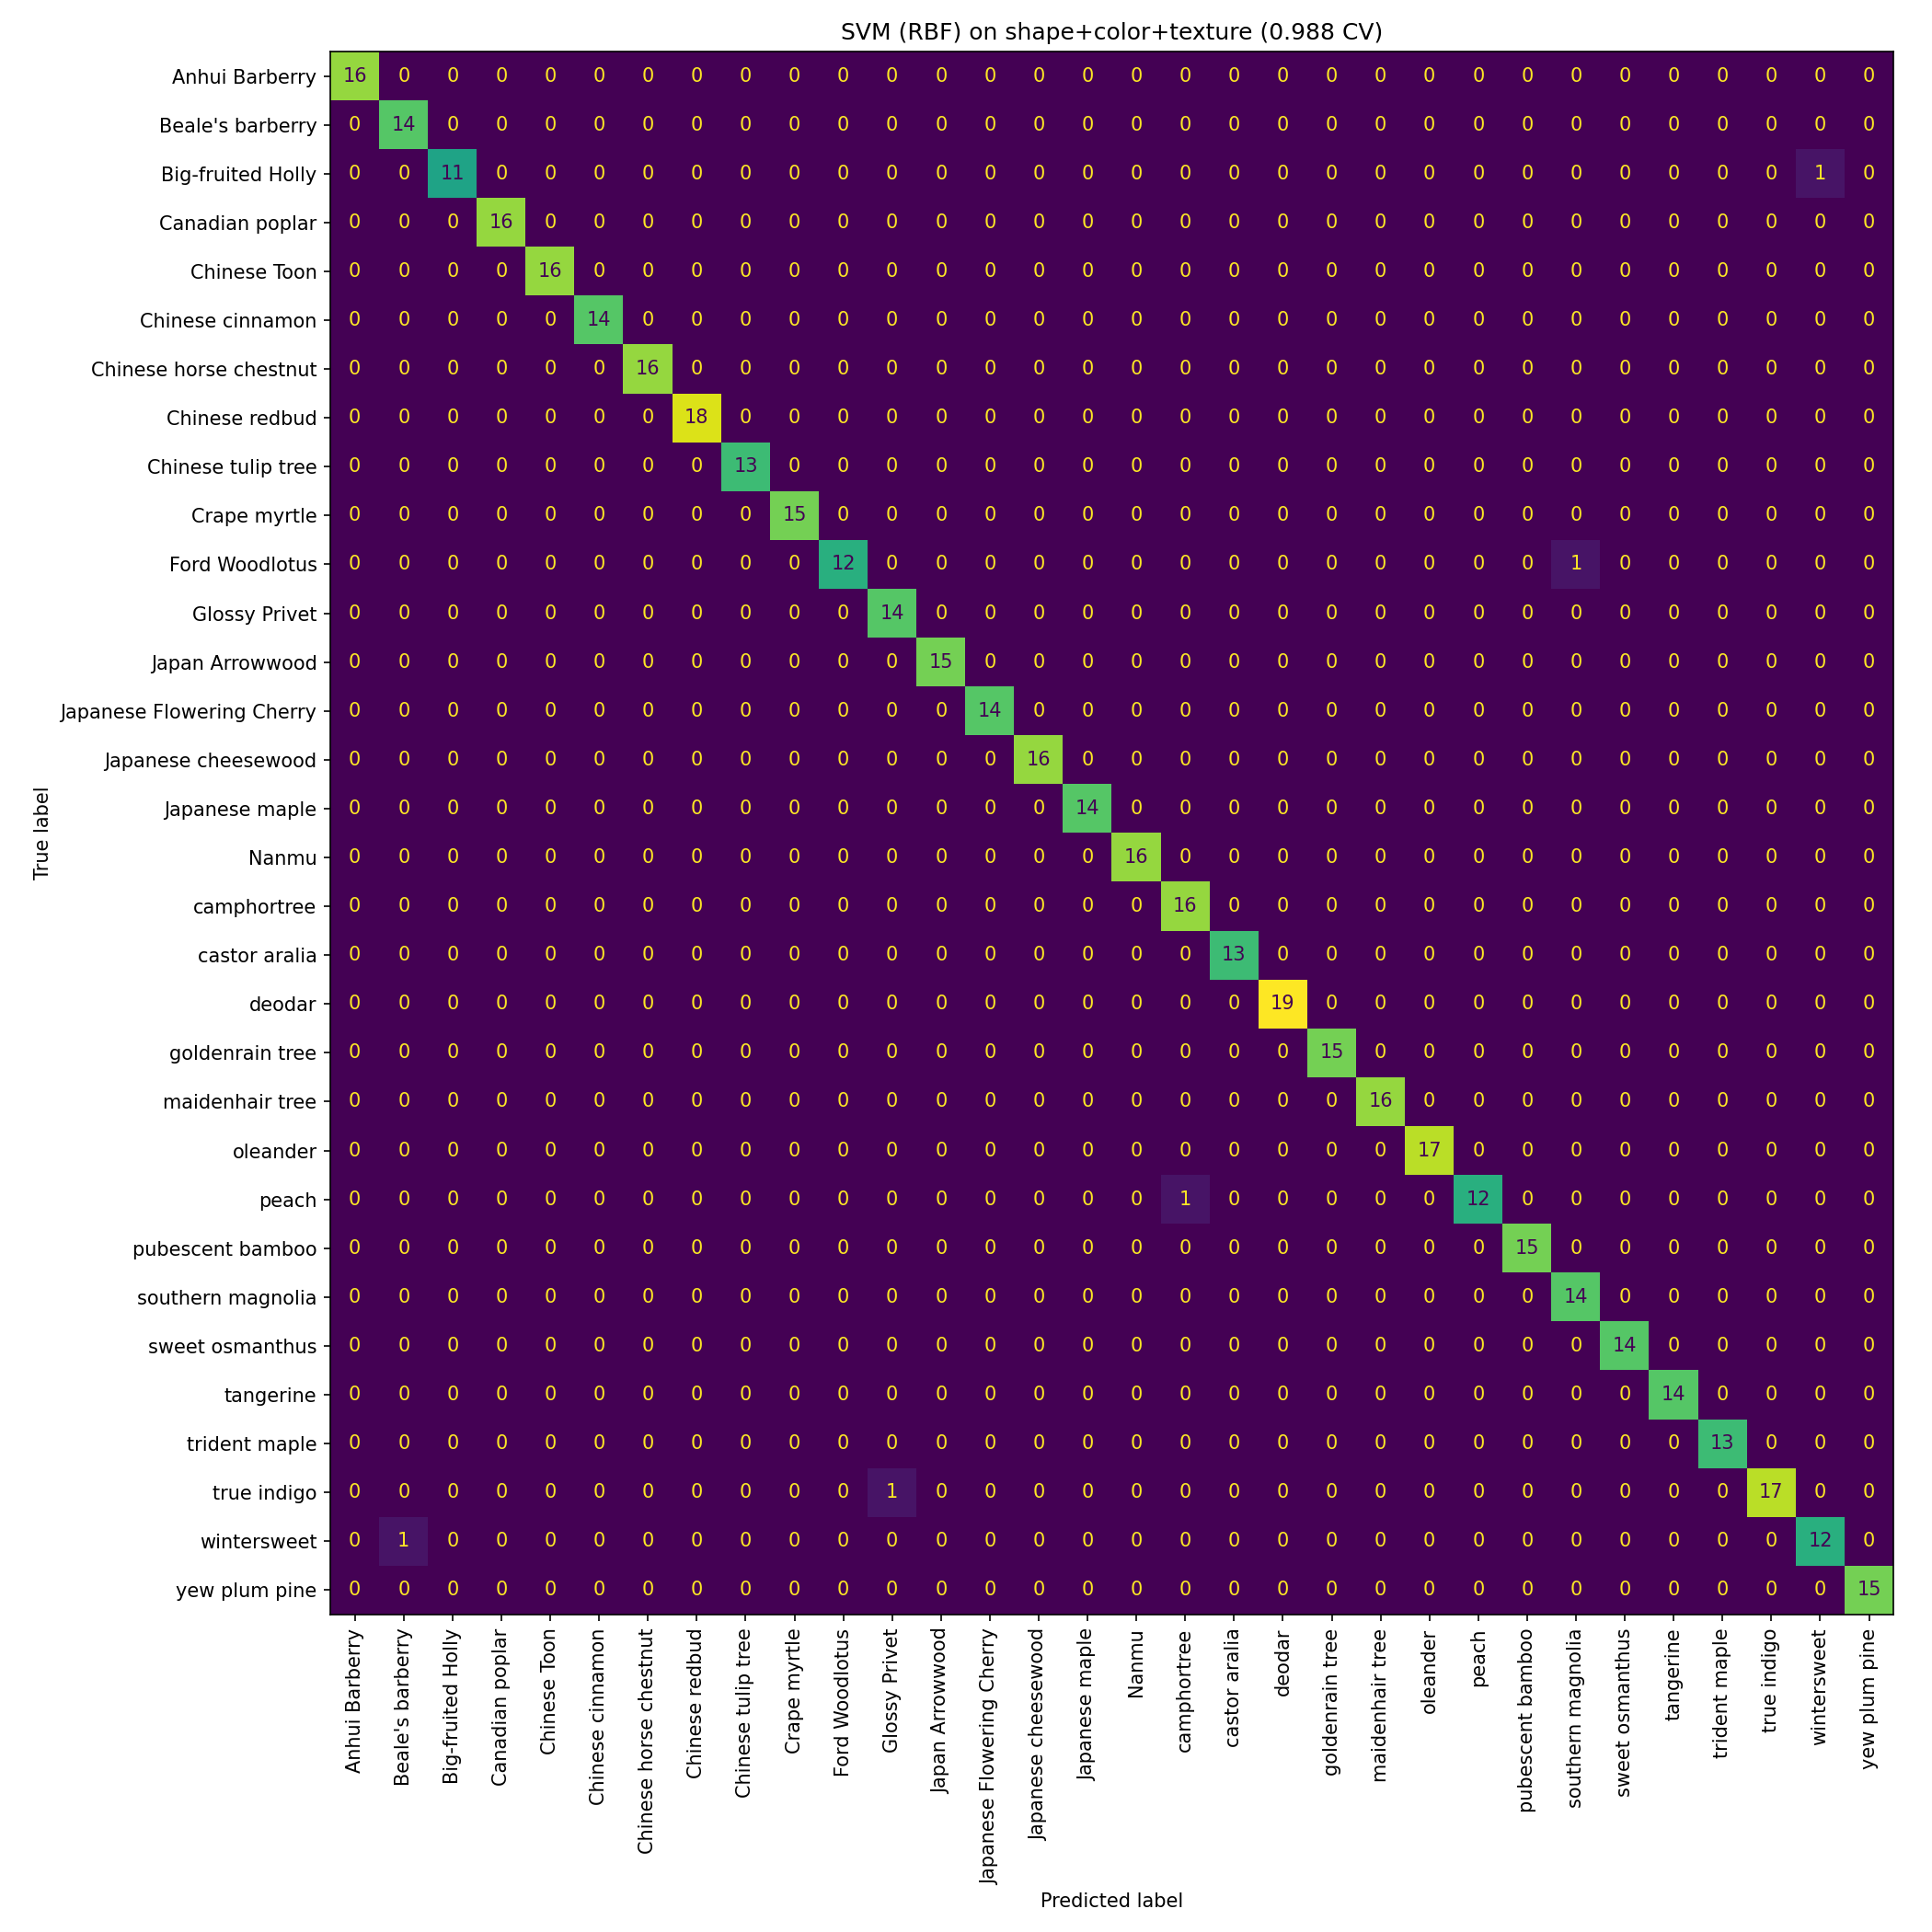
\includegraphics[width=0.9\linewidth]{confusion.png}
  \caption{Ma trận nhầm lẫn trên tập kiểm tra giữ lại (25\% dữ liệu) của cấu hình tốt nhất
  (\holdouterrors{}/\holdouttotal{} mẫu bị phân lớp sai, liệt kê ở Bảng~\ref{tab:errors}).}
  \label{fig:confusion}
\end{figure}

\end{document}
